\chapter{Large Language Models}

\vspace{1em}
\hfill
\begin{minipage}[c]{0.65\textwidth}
\raggedleft
\small\itshape
General methods that leverage computation are ultimately the most effective, and by a large margin.\\[0.5em]
\upshape\footnotesize Richard Sutton, ``The Bitter Lesson'' (2019)
\end{minipage}
\vspace{1.5em}

\noindent Part III is closed. The mathematics of optimal agency is built; the specification problem is named; the structural argument for why optimization is dangerous is on the page; the mitigations and their limits are mapped.

Part IV is about the practice. The system that everyone in 2026 has encountered, that has driven the public conversation about AI for several years, that is the empirical face of the technical argument the book has built up to: the large language model.

This chapter does two things. The first half traces how we got here, because the trajectory is the cleanest way for a reader to feel where we are. The second half says what a base language model actually is, mathematically, and connects it to the apparatus from Parts I and II.

The next chapter, on reward and reasoning, covers how a base model is turned into the assistants and agents of 2026: fine-tuning, the reward signals that can and cannot be trusted, and the inference-time compute that drives the reasoning models. Chapter 15 then names the gap between what an LLM actually does and what AIXI says optimal agency would do, Chapter 16 asks where the trajectory is going, and the final chapter lays out the stakes.

\section*{The horizon}

A useful question to ask of any AI system is: how long can it work on a task before it fails or needs help?

A human looking at a photograph and saying ``that's a cat'' takes about a second. A human writing a short email takes a few minutes. A human debugging a moderately complex bug in a codebase they have not seen before takes hours. A human shipping a small but real software feature, end to end, takes a day.

These are not strict task categories. They are a way of measuring how much sustained, coherent, correct work a system can do without falling off the rails.

Roughly, here is the trajectory.

In 2013, the answer for the best AI systems was about a second. Image classification at near-human accuracy was the frontier; multi-step reasoning, planning, anything that compounded errors over time, was beyond reach.

In 2026, the answer is in the range of an hour to a day for the right kind of task, given the right scaffold. METR (Kwa et al.\ 2025) measured this directly, on a benchmark of programming-style tasks. The time-horizon of a task that a frontier system can complete reliably has been roughly doubling every seven months across the 2019 to 2025 window, and the doubling appears to have sped up to around every four months over 2024 and 2025. The figure is worth treating with care: it is measured on a specific suite of software and reasoning tasks under controlled conditions, it is the horizon at a fifty-percent success rate, and METR itself has cautioned that the longest estimates are the least reliable and that the number does not translate directly into autonomous real-world work. With those caveats, the direction is not in doubt. If the trend continues (a real ``if''), the next several years extend the horizon to weeks and beyond.

Time-horizon is a useful summary statistic because it folds two things into one number a reader can hold: capability (how hard a task the system can do at all) and reliability (how often it does the task without derailing). Doing a hard task once, with luck, is not the same as doing it again and again at length. Pushing the horizon out requires gains in both, at once. The trajectory is the trajectory of both gains together.

The rest of this section is the history of how the horizon was extended.

\section*{A short history}

\textbf{2012: AlexNet on ImageNet.} Krizhevsky, Sutskever, and Hinton entered the ImageNet Large Scale Visual Recognition Challenge with a deep convolutional neural network trained on GPUs. They beat the field by a margin so large that the field reorganized around the result. Object recognition in still images, the second-scale perceptual problem, was solved well enough to deploy. Deep learning, after years on the academic margins, became the way to do perception. (The earlier MNIST handwriting benchmark had been solved by simpler methods; ImageNet was the result that mattered, because the task was natural images at scale.)

\textbf{2016: AlphaGo.} DeepMind's program defeated Lee Sedol at Go in a five-game match in Seoul. The technical recipe combined two things: a deep convolutional network trained to evaluate positions and propose moves (the policy and value networks), and Monte Carlo Tree Search at inference time using those networks as guides. The lesson was not just that Go fell. It was that spending compute at inference time, not only at training time, is one of the things general methods do. AlphaGo Zero (2017) extended the recipe to learn from self-play with no human data; AlphaZero (2017) generalized it to chess and shogi at the same level.

\textbf{2019: AlphaStar.} DeepMind reached grandmaster level at StarCraft II, a real-time strategy game with partial information, long-horizon planning, and continuous time pressure. The horizon extended to minutes of coherent play, in a setting where humans had assumed they had structural advantages of intuition and macro-management.

\textbf{2019: GPT-2.} OpenAI scaled up a transformer-based language model and trained it on a large sample of web text using next-token prediction. The surprise was the quality of the generated text: multi-paragraph passages that were coherent at the paragraph level, sometimes factual, often confabulated. OpenAI initially declined to release the largest version, citing misuse concerns. That decision became controversial, but the underlying observation, that scaling next-token prediction produces unexpectedly capable systems, drove the next several years.

\textbf{2020: GPT-3.} OpenAI scaled further, to 175 billion parameters. The surprise this time was \emph{in-context learning}. Show the model a few examples of a task in the prompt, and it would do the task without any parameter updates. The horizon was now short multi-step tasks the model had never explicitly been trained on, performed by inferring the task from a few examples. Brown et al.\ titled the paper \textit{Language Models are Few-Shot Learners}; that title captured what had changed.

\textbf{2022: ChatGPT.} OpenAI released a conversational interface to GPT-3.5, the model fine-tuned with RLHF (reinforcement learning from human feedback) to follow instructions and be helpful. The product reached 100 million users in about two months, the fastest consumer-software adoption in history at the time. The horizon was an interactive conversation: a few turns of back-and-forth, repeated. The public conversation about AI changed in those months and has not changed back.

\textbf{2023: GPT-4.} OpenAI's GPT-4 was the capability jump that made even careful observers reorient. It passed bar exams, AP exams, the GRE quantitative section, and a substantial range of professional certification tests, often in the top deciles. Multi-step reasoning held together better. Code generation became useful enough that practicing engineers started incorporating it into their workflows. The horizon extended from ``answer a question'' to ``carry a chain of reasoning across a page.''

\textbf{2023 onward: the frontier becomes plural.} Anthropic released Claude. Google DeepMind released Gemini. Meta released Llama with open weights. Mistral, DeepSeek, xAI, and others entered. Cross-pollination of techniques meant that capability advances at one lab tended to appear at others within months. The open-weight families, especially Llama and later DeepSeek, narrowed the gap between the proprietary frontier and what anyone could run locally.

\textbf{2024 onward: reasoning models.} OpenAI's o1, then o3. DeepSeek's R1. Anthropic's extended-thinking modes. These systems are trained with reinforcement learning on problems whose solutions can be verified: mathematics, code, formal logic. At inference time, they generate long chains of thought, sometimes sampling many trajectories and selecting among them. The capability jump on math and code benchmarks was large enough that some benchmarks had to be retired, the top models saturating them within months of release. The horizon on a verifiable task extended from minutes to hours.

\textbf{2024-2025: scaffolded agents.} Claude Code, Cursor, Devin, Replit Agent, and others. The pattern: an LLM embedded in a loop that can read files, edit files, run commands, observe outputs, decide what to do next, and iterate. The model is the same kind of thing it always was; the loop is what is new. METR's task-length benchmark put the current frontier around the day mark for some programming tasks, the kind of work that would take a competent human engineer a full working day to complete.

The trajectory in one line: a second in 2013, a day in 2026. Figure~\ref{fig:horizon-timeline} lays the milestones on a single axis. Whatever the right extrapolation is, the trend has held for over a decade.

\begin{figure}[h]
\centering
\begin{tikzpicture}[
  every node/.style={align=center},
  >=Stealth
]
  \draw[->, thick, gray] (-0.2, 0) -- (11.0, 0);

  \draw[thick] (0.4, -0.08) -- (0.4, 0.08);
  \node[anchor=south, yshift=2pt, font=\scriptsize] at (0.4, 0.08) {AlexNet};
  \node[anchor=north, font=\tiny] at (0.4, -0.12) {2012};
  \node[anchor=north, font=\tiny, gray, yshift=-9pt] at (0.4, -0.12) {\itshape sec};

  \draw[thick] (2.0, -0.08) -- (2.0, 0.08);
  \node[anchor=south, yshift=2pt, font=\scriptsize] at (2.0, 0.08) {AlphaGo};
  \node[anchor=north, font=\tiny] at (2.0, -0.12) {2016};
  \node[anchor=north, font=\tiny, gray, yshift=-9pt] at (2.0, -0.12) {\itshape game};

  \draw[thick] (3.8, -0.08) -- (3.8, 0.08);
  \node[anchor=south, yshift=2pt, font=\scriptsize] at (3.8, 0.08) {GPT-2,\\AlphaStar};
  \node[anchor=north, font=\tiny] at (3.8, -0.12) {2019};
  \node[anchor=north, font=\tiny, gray, yshift=-9pt] at (3.8, -0.12) {\itshape min};

  \draw[thick] (5.7, -0.08) -- (5.7, 0.08);
  \node[anchor=south, yshift=2pt, font=\scriptsize] at (5.7, 0.08) {ChatGPT};
  \node[anchor=north, font=\tiny] at (5.7, -0.12) {2022};
  \node[anchor=north, font=\tiny, gray, yshift=-9pt] at (5.7, -0.12) {\itshape conv};

  \draw[thick] (7.2, -0.08) -- (7.2, 0.08);
  \node[anchor=south, yshift=2pt, font=\scriptsize] at (7.2, 0.08) {GPT-4};
  \node[anchor=north, font=\tiny] at (7.2, -0.12) {2023};
  \node[anchor=north, font=\tiny, gray, yshift=-9pt] at (7.2, -0.12) {\itshape page};

  \draw[thick] (8.9, -0.08) -- (8.9, 0.08);
  \node[anchor=south, yshift=2pt, font=\scriptsize] at (8.9, 0.08) {o1, R1};
  \node[anchor=north, font=\tiny] at (8.9, -0.12) {2024};
  \node[anchor=north, font=\tiny, gray, yshift=-9pt] at (8.9, -0.12) {\itshape hour};

  \draw[thick] (10.6, -0.08) -- (10.6, 0.08);
  \node[anchor=south, yshift=2pt, font=\scriptsize] at (10.6, 0.08) {agents};
  \node[anchor=north, font=\tiny] at (10.6, -0.12) {2025-26};
  \node[anchor=north, font=\tiny, gray, yshift=-9pt] at (10.6, -0.12) {\itshape day};
\end{tikzpicture}
\caption{The horizon trajectory. Each milestone, with the rough time-horizon of the task it could do (italicized below the year). The units across paradigms (image classification, game-play, conversation, agentic task) are not strictly comparable, but the direction is unmistakable. ChatGPT (2022) introduced RLHF as the dominant fine-tuning method; o1 and R1 (2024) introduced RLVR. METR (Kwa et al.\ 2025) finds the time-horizon on programming-style tasks roughly doubling every seven months over 2019 to 2025, accelerating to about every four months in 2024 to 2025.}
\label{fig:horizon-timeline}
\end{figure}

\section*{What an LLM is}

The dominant system on the frontier in 2026 is the large language model. Strip away the chat interface, the tool-use scaffolding, the multi-modal additions, and the underlying object is straightforward to describe.

An LLM parameterizes a conditional distribution

$$p_\theta(x_t \mid x_{<t})$$

over the next token $x_t$ in a sequence, given the previous tokens $x_{<t}$. A token is a word or word fragment from a fixed vocabulary (typically about 100,000 tokens). The parameters $\theta$ are the weights of a deep neural network, on the order of $10^{11}$ to $10^{12}$ of them for a frontier model.

The training objective is the cross-entropy loss

$$\mathcal{L}(\theta) = -\mathbb{E}_{x \sim \text{data}}\sum_t \log p_\theta(x_t \mid x_{<t}).$$

The expectation is over a vast text corpus: most of the internet's text, books, code repositories, scientific papers. Training minimizes the average negative log probability the model assigns to the actual next token in real text. Up to a constant, this is the average number of bits needed to encode the next token under the model's distribution (Chapter 3). Better predictions; fewer bits; lower loss.

The architecture is the transformer (Vaswani et al.\ 2017). Figure~\ref{fig:transformer-block} sketches one block.

\begin{figure}[h]
\centering
\begin{tikzpicture}[
  scale=0.85,
  every node/.style={align=center, font=\small},
  >=Stealth
]
  \node[font=\scriptsize, anchor=south] (input) at (0, 0) {input: token embeddings};
  \draw[->, thick] (0, 0.1) -- (0, 0.7);

  \node[draw, fill=gray!10, rounded corners, minimum width=3.5cm, minimum height=0.5cm] (ln1) at (0, 1) {layer norm};
  \draw[->, thick] (0, 1.3) -- (0, 1.8);

  \node[draw, fill=blue!20, rounded corners, minimum width=3.5cm, minimum height=0.8cm] (attn) at (0, 2.2) {multi-head\\self-attention};
  \draw[->, thick] (0, 2.6) -- (0, 3.1);

  \node[draw, circle, fill=white, inner sep=2pt] (add1) at (0, 3.3) {\scriptsize $+$};
  \draw[thick] (1.75, 0.6) -- (2.5, 0.6) -- (2.5, 3.3) -- (0.2, 3.3);
  \node[font=\tiny, gray, anchor=west] at (2.6, 1.95) {residual};

  \draw[->, thick] (0, 3.5) -- (0, 4.0);

  \node[draw, fill=gray!10, rounded corners, minimum width=3.5cm, minimum height=0.5cm] (ln2) at (0, 4.25) {layer norm};
  \draw[->, thick] (0, 4.5) -- (0, 5.0);

  \node[draw, fill=green!20, rounded corners, minimum width=3.5cm, minimum height=0.8cm] (ff) at (0, 5.4) {feed-forward\\network};
  \draw[->, thick] (0, 5.8) -- (0, 6.3);

  \node[draw, circle, fill=white, inner sep=2pt] (add2) at (0, 6.5) {\scriptsize $+$};
  \draw[thick] (-1.75, 3.85) -- (-2.5, 3.85) -- (-2.5, 6.5) -- (-0.2, 6.5);
  \node[font=\tiny, gray, anchor=east] at (-2.6, 5.2) {residual};

  \draw[->, thick] (0, 6.7) -- (0, 7.2);
  \node[font=\scriptsize, anchor=north] at (0, 7.4) {output to next block};
\end{tikzpicture}
\caption{One transformer block. Input flows upward through layer normalization, multi-head self-attention (every position reads from every other position with learned weights), another layer norm, and a feed-forward network. Residual side wires carry the input around each sub-block and add it back. A full model stacks dozens to over a hundred such blocks.}
\label{fig:transformer-block}
\end{figure}

The central operation is attention. At each position in the sequence, the representation is updated by reading from every other position with learned weights, where the weights are computed from a similarity between queries and keys at each position. Multi-head attention runs this in parallel with several different projections, letting different heads pick up different patterns. Feed-forward sub-blocks apply position-wise nonlinear transforms. Residual connections (the side wires) let the network learn small modifications to a running representation rather than rebuilding it from scratch. Most of the parameters live in the feed-forward sub-blocks; the long-range structure comes from attention.

The third piece is scaling. Kaplan et al.\ (2020) measured that the loss decreases as a power law in parameters, data, and compute, holding the others fixed. Hoffmann et al.\ (2022, the Chinchilla result) refined the picture: for a fixed compute budget, there is an optimal trade-off between parameters and data, and the earlier models had been over-parameterized relative to their training data. Frontier models in 2025-2026 are built to Chinchilla-style compute-optimality or its successors.

The structural fact that drives industrial AI investment is that the cost-to-capability curve is smooth. Doubling compute, with data scaled appropriately, produces a predictable amount of additional capability. Sutton's bitter lesson is the recurring methodological observation; scaling laws are the quantitative version.

\section*{What the architecture commits to}

The previous section described what a transformer mechanically is. The harder question, and the one that matters for everything Part IV says about the gap, is what the architecture commits to about the data. Architecture is inductive bias (Chapter 7). The transformer's biases are not arbitrary; each one is a claim about what kind of structure the data has.

Four commitments are load-bearing.

\textbf{Long-range as cheap.} Every position in the sequence can attend directly to every other position. A convolutional network builds its receptive field gradually through depth; a one-layer CNN sees only locally. A recurrent network can in principle attend over arbitrary distances but in practice struggles to retain information across many steps. A transformer's attention is global from the first layer. This matches language, where a pronoun can refer to a noun many sentences earlier, where the meaning of an early phrase depends on something much later, and where the structure of an argument crosses paragraph boundaries. Figure~\ref{fig:info-flow} compares the three connectivity patterns.

\begin{figure}[h]
\centering
\begin{tikzpicture}[
  scale=1.0,
  every node/.style={font=\scriptsize},
  >=Stealth
]
  % CNN row
  \node[font=\small\bfseries, anchor=east] at (0.4, 5) {CNN};
  \foreach \x/\fill in {1/white, 2/white, 3/blue!20, 4/blue!50, 5/blue!20, 6/white, 7/white} {
    \node[draw, minimum size=6mm, fill=\fill] at (\x, 5) {};
  }
  \node[anchor=west, font=\scriptsize, gray] at (7.8, 5) {local window};

  % RNN row
  \node[font=\small\bfseries, anchor=east] at (0.4, 3.7) {RNN};
  \foreach \x/\fill in {1/blue!8, 2/blue!15, 3/blue!25, 4/blue!50, 5/white, 6/white, 7/white} {
    \node[draw, minimum size=6mm, fill=\fill] at (\x, 3.7) {};
  }
  \node[anchor=west, font=\scriptsize, gray] at (7.8, 3.7) {chain, fading};

  % Transformer row
  \node[font=\small\bfseries, anchor=east] at (0.4, 2.4) {Transformer};
  \foreach \x/\fill in {1/blue!35, 2/blue!35, 3/blue!35, 4/blue!50, 5/white, 6/white, 7/white} {
    \node[draw, minimum size=6mm, fill=\fill] at (\x, 2.4) {};
  }
  \node[anchor=west, font=\scriptsize, gray] at (7.8, 2.4) {all past, equally};
\end{tikzpicture}
\caption{Information flow after one layer, under causal structure. Each row is a sequence of seven tokens; position 4 (the focal token, darker) shows the receptive field of each architecture. CNN sees only a local window. RNN can in principle reach all earlier positions but information from early ones degrades with distance. Transformer's attention reads all earlier positions in one operation, with no positional decay. ``Global from layer 1'' is the load-bearing property.}
\label{fig:info-flow}
\end{figure}

\textbf{Soft retrieval over learned similarity.} Attention is, mathematically, a learned form of kernel regression: the output at each position is a weighted average of values, with weights given by a learned similarity function between queries and keys. This is a primitive operation that supports pattern-matching across context. Mechanistic interpretability has identified specific transformer circuits, the \emph{induction heads} of Olsson et al.\ (2022), that implement exactly this in trained models: when the model has seen the pattern $\ldots A B \ldots$ earlier and now sees $A$ again, the circuit looks back, finds the previous $A$, and uses what followed it to predict the next token. The architecture provides the substrate; training discovers how to use it.

\textbf{Causal masking.} A decoder-only transformer (the dominant LLM architecture in 2026) restricts attention to be causal: a position can attend only to itself and earlier positions, not to the future. This is a commitment about the data: the joint distribution factors as $p(x_1) p(x_2 \mid x_1) p(x_3 \mid x_{1:2}) \cdots$, an autoregressive structure where future tokens depend on past, not the other way around. This matches language (we write past-to-future) and any generative process with an arrow of time. It is the wrong commitment for tasks without a natural causal order, which is why bidirectional architectures (BERT-style encoders) coexist for understanding tasks even though they are niche compared to decoder-only generation. Figure~\ref{fig:attention-masks} shows the difference.

\begin{figure}[h]
\centering
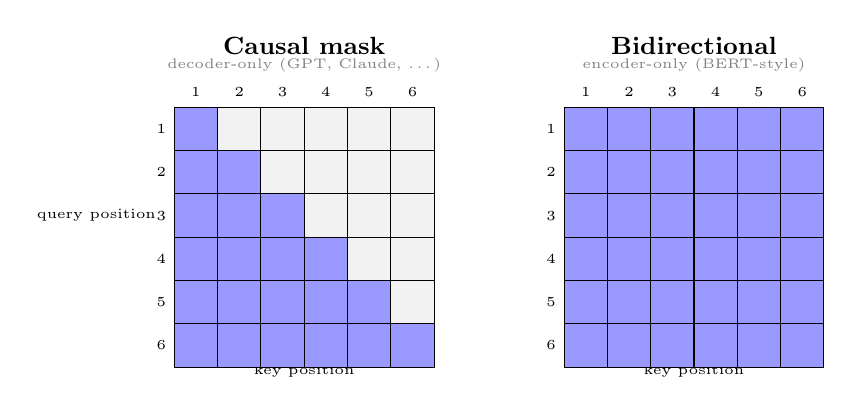
\begin{tikzpicture}[scale=0.55, every node/.style={font=\scriptsize}]
  % Causal mask (left)
  \node[font=\small\bfseries, anchor=south] at (3, 6.5) {Causal mask};
  \node[font=\tiny, anchor=south, gray] at (3, 6.1) {decoder-only (GPT, Claude, \ldots)};
  \node[font=\tiny, anchor=east] at (-0.2, 3) {query position};
  \node[font=\tiny] at (3, -0.6) {key position};
  \foreach \i in {1,...,6} {
    \node[font=\tiny] at (\i-0.5, 5.85) {\i};
    \node[font=\tiny] at (-0.3, 5.5-\i+0.5) {\i};
  }
  \foreach \i in {1,...,6} {
    \foreach \j in {1,...,6} {
      \pgfmathparse{int(\j <= \i)}
      \ifnum\pgfmathresult=1
        \draw[fill=blue!40] (\j-1, 5.5-\i) rectangle (\j, 5.5-\i+1);
      \else
        \draw[fill=gray!10] (\j-1, 5.5-\i) rectangle (\j, 5.5-\i+1);
      \fi
    }
  }

  % Bidirectional (right)
  \node[font=\small\bfseries, anchor=south] at (12, 6.5) {Bidirectional};
  \node[font=\tiny, anchor=south, gray] at (12, 6.1) {encoder-only (BERT-style)};
  \node[font=\tiny] at (12, -0.6) {key position};
  \foreach \i in {1,...,6} {
    \node[font=\tiny] at (\i+8.5, 5.85) {\i};
    \node[font=\tiny] at (8.7, 5.5-\i+0.5) {\i};
  }
  \foreach \i in {1,...,6} {
    \foreach \j in {1,...,6} {
      \draw[fill=blue!40] (\j+8, 5.5-\i) rectangle (\j+9, 5.5-\i+1);
    }
  }
\end{tikzpicture}
\caption{Attention masks. Each matrix shows which positions (columns, keys) can be attended to by which positions (rows, queries). Causal mask (left): a position attends only to itself and earlier positions; the lower triangle plus diagonal are open. Bidirectional (right): every position attends to every other; the full matrix is open. Decoder-only LLMs commit to autoregressive structure; encoder-only models (now niche) suit understanding tasks where the full input is available.}
\label{fig:attention-masks}
\end{figure}

\textbf{Compositional layered processing.} Stacked attention-and-feedforward blocks let representations be built up in layers. Shallow layers handle local processing (token-level features, simple syntactic patterns); deeper layers do more abstract synthesis (reasoning patterns, world knowledge, discourse structure). The residual stream connecting them serves as a kind of workspace: each layer reads from it, adds to it, and passes it forward. This matches the compositional hierarchy of language itself, from phonemes through words through phrases through documents.

Those four commitments together are most of why transformers fit language. Language has long-range dependencies, depends on pattern-matching across context, has an arrow of time, and has compositional hierarchy. The architecture was an empirical bet that those four biases were the right ones for human text. The scaling laws of the last decade are the bet paying off.

What is still genuinely not understood at the level of theory: why these specific biases produce the emergent capabilities they do at scale, why the loss decreases as the particular power law it does, why scaling produces something that behaves like a world model rather than a larger surface-statistics table. The architecture works. The theoretical account of why is still being developed; the empirical results are running ahead of the explanations.

\section*{The Solomonoff connection}

The reader who has worked through Parts I and II has the framework to see what an LLM is in conceptual terms.

It is a parameterized function approximator (Chapter 7) with the four commitments above, applied to sequences of tokens from human text. Its output at each position is a softmax distribution over the vocabulary: a probability distribution over what comes next, not a point prediction. Training minimizes the cross-entropy of that distribution against the empirical next-token distribution in the data.

That training objective is, structurally, four things at once. It is \emph{maximum likelihood estimation}: choose the parameters $\theta$ that make the training data most probable under the model. It is \emph{cross-entropy minimization}: drive the model's distribution toward the data's distribution. It is \emph{Shannon-coding minimization} (Chapter 3): minimize the average bits needed to encode the data under the model's distribution. And it is a \emph{bounded approximation to conditioning Solomonoff's universal prior $M(x_t \mid x_{<t})$ on the prefix} (Chapter 4). Four perspectives, from statistics, information theory, source coding, and algorithmic information theory; one procedure, which is the procedure that trains every base language model in 2026. The traditions converge because they were always describing the same object: the probability distribution that best matches the data.

A subtlety the precise reader will catch. The four perspectives converge on the \emph{training procedure}, not on the inference behavior. MLE picks a single best $\theta$. A real Bayesian treatment, of which Solomonoff is the universal-prior case, would maintain a posterior over parameters and therefore a distribution over distributions. Solomonoff is not one distribution; it is a Bayesian mixture over all computable distributions $\nu$, weighted by $2^{-K(\nu)}$, with posteriors updated by Bayes' rule as data arrives. The LLM collapses this to a point estimate. So the LLM is a bounded approximation to Solomonoff in two ways, not one: bounded function class (the transformer can represent only a subset of computable hypotheses) and bounded inference (point estimate via MLE rather than the full posterior). Both contribute to the gap from optimal.

The data side of the system is itself an inductive bias. Human text comes with structure encoded by humans at every level: morphology, syntax, semantics, discourse, rhetoric, argument structure. The model is not discovering structure from scratch in a high-entropy environment; it is learning to model regularities that humans put there on purpose in producing the text. This is part of why pretraining is so much more than ``more training'': the data provides pre-organized patterns at the right level of abstraction for downstream tasks. The same architecture trained on raw sensor data or molecular dynamics simulations would have to discover its regularities from much less pre-structured inputs, and the transformer's biases might not be the right ones for that case. The composition of architecture, data, and objective is what produces what we see; the architecture alone would not have done it.

The function class is bounded. The data is bounded. The prior is whatever the architecture and training distribution implicitly impose. None of this is Solomonoff. All of it is the same conceptual object Solomonoff is the limit of.

What is surprising, and what most of the recent decade was about, is how well the bounded approximation does. The Solomonoff connection makes a soft prediction: a sufficiently capable approximator trained on enough data should converge toward the structure of the data-generating process. Human text is generated by humans thinking, which is generated by brains, which are bounded but rich computational systems. An LLM that fits human text well must learn an approximation of whatever computational regularities make human text predictable. Those regularities apparently include grammar, world knowledge, conversational structure, common reasoning patterns, mathematical notation, and code. They include enough of how humans frame problems for the model to imitate the framing convincingly.

This is the conceptual payoff Parts I and II were aiming at. LLMs are not Solomonoff. They are the closest practical realization of the same conceptual object the world has ever built. The math of Parts I and II is not idle theory. It describes the family of systems the LLM lives in.

\section*{Where this leaves you}

You have half of what an LLM is.

A base language model is a bounded function approximator (Chapter 7), built on the transformer's four commitments, trained on human text by next-token prediction. That training is, at once, maximum likelihood estimation, cross-entropy minimization, Shannon-coding minimization, and a bounded approximation to conditioning Solomonoff's universal prior on the prefix (Chapters 3 and 4). It is the closest practical realization of the conceptual object Parts I and II were built around, and it is not Solomonoff: the function class is bounded, the inference is a point estimate, and the prior is whatever the architecture and data impose.

What a base model is, though, is a predictor. It continues text. On its own it does not answer questions helpfully, follow instructions, write working code on request, or carry a task across a working day. The systems that do those things are base models that have been fine-tuned, given reward signals, and wrapped in loops that let them act and check their own work. That is the other half of what an LLM is in 2026, and it is where the specification problem of Part III walks back onto the stage.

The next chapter is about reward and reasoning: how a predictor becomes an agent, which reward signals can be trusted under optimization and which cannot, and why the strongest systems of the reasoning-model era are the ones that found a reward they could not game.
